\chapter{Detecting crucial parts in inputs}
\label{cha:3:intro}
When we detect that the PUT crashes, wrongly satisfies, wrongly unsatisfies, hangs or gives the wrong solution on a given input we want to know why it does that. What causes this unwanted output and on what line the bug occurs. With crashes, a stack trace and some luck this could be easy, but when a bug causes a crash in another place or we get another unwanted output the developer may need to debug deep into the code to find the bug. This with a potential large inputs created by the fuzzer could be a tedious and long assignment, for this reason we would like to know what parts of the input are related to the bug. We will discover this further in this chapter, starting with deobfuscating inputs.
\todo{algorithms? paper 5 has nice simplification to isolation delta deb, called 'ddmin()'}

\section{Deobfuscating inputs}
\label{cha:3:Deobfuscating}
When receiving a big input the chance of it having parts unrelated to the bug is almost guaranteed, we will call these inputs (unintentionally) obfuscated inputs. Deobfuscating those takes a lot of trying parts of the inputs to see if the bugs are still there \cite{bookZellerwhyProgramsFail} or having to walk through the execution to find the bugs. Both take a while if we want to go to absolute minimal inputs, but for developers it is not needed to go to that extreme. As long as we take the bulk of the unrelated parts of inputs away it will help the developer to find the bug faster. With these techniques we can also group similar bugs and duplicate errors (more on that later) which is also fairly useful information for developers.
\subsection{Simplifying}
\label{cha:3:Simplifying}
To find crucial parts of inputs, it is often achieved either with simplification or Isolation. 
Simplification is the technique where we repeatably remove parts of a failing input and check if it still fails and it often called "delta-debugging" \cite{bookZellerwhyProgramsFail}, which belongs to the divide-and-conquer family of algorithms \cite{2FuzzingAndDeltaDebuggingSMTSolvers}. 
When it is no longer possible to remove any part of the input we have obtained an input where all parts are necessary to expose the bug. This input is at the same time also the shortest possible input to trigger this bug, making finding the bug easier than in the original input filled with unrelated parts.

\subsection{Isolation}
\label{cha:3:Isolation}
The second technique, isolation, is a technique where instead of minimizing the input we try to find the smallest difference between an input that shows the bug versus an input that does not show the bug. This with the advantage that no matter if we find the bug or not the difference will diminish, either the maximum input will shrink or the minimum input will grow. 
This technique brings extra complexity with the tracking of multiple inputs and bigger inputs often take longer, but according to Andreas Zeller et al. \cite{5zeller2002simplifyingIsolatingFailure-inducing} this is the faster one to the two techniques. 
Figure \ref{fig:simplificationIsolation} shows the difference between simplifying and isolation both finding the critical part of the input. With simplification the critical part is indicated by the last test in the figure while with isolation it is the difference of the last passed and last failed tests.
\begin{figure}
	\centering
	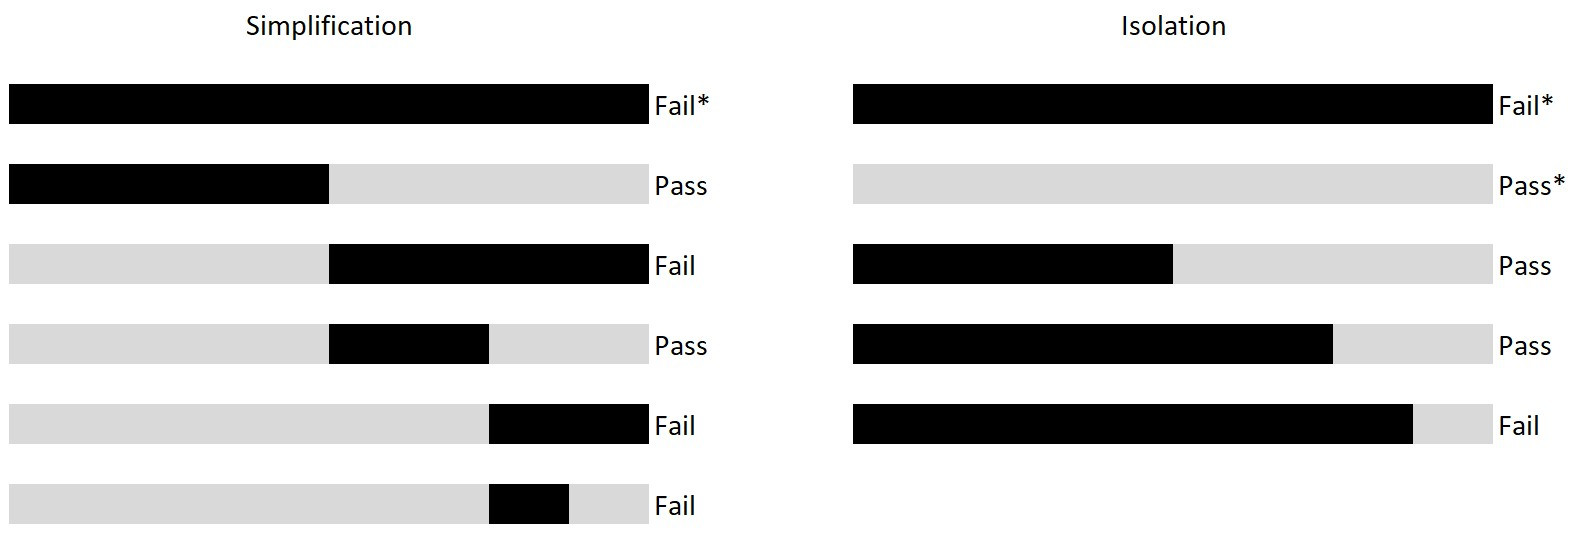
\includegraphics[width=1.0\textwidth]{images/simplificationIsolation}
	\caption{Deobfuscating inputs based on simplification (left) and isolation (right) on the same input. The '*' indicates that the result is already known and does not need to be recalculated. Figure based on an illustrations found in Why programs fail: a guide to systematic debugging by Andreas Zeller \cite{bookZellerwhyProgramsFail}.}
	\label{fig:simplificationIsolation}
\end{figure}

\subsection{Connection with minimal unsatisfiable subset and maximally satisfiable subsets}
For readers that are familiar with the SMT of constraint solving-world will have noticed that this techniques feels similar to a way of finding the minimal unsatisfiable subset (MUS), which it is in the case of a solver (wrongly) stating that an input is unsatisfiable. With MUS you try to find the smallest subset of formulas (or constraints) that will result in an unsatisfiable solution while with MSS you would be trying to find the biggest set of formulas (or constraints) that would result in a satisfiable solution. Both are an iterative process and can be applied in the simplification and the isolation process. But solving which combination of formulas results in the smallest of biggest subset is an computationally intensive progress. Fortunately a lot ot though has already been put in it to reduce it, for example Mark H. Liffiton et al. have proposed multiple "Algorithms for Computing Minimal Unsatisfiable Subsets of Constraints" \cite{51liffiton2008algorithms}. Again we should note that an Minimal input is not needed as we aim to reduces de input to help de developer find the error faster, a difference between a smaller and the absolute minimum will cause for a big difference in practice.


\subsection{Alternative approach}
An alternative approach compared to the already mentioned techniques is one by Alexandra Bugariu and Peter M\"uller \cite{9bugariu2020automaticallyTestingStringSolvers} is to forgo the need of deobfuscating inputs by generating inputs "small by construction". Because the smaller the inputs are the space there is for remaining stuff to obfuscate the Input. On the other hand the chance of finding bigger bugs with multiple constraints interacting with each other will be harder to find.
A last alternative approach would be retrying fuzzing by adding an increasing size limitation to find the same bug input as done by Muhammad Numair Mansur et al \cite{1mansur2020detecting}.

\section{What size to change}
\label{cha:3:Chucksize}
A subject we glossed over is the chuck size, the size to remove while trying to find the critical parts of the inputs. 
The previous seen techniques will work well on the original fuzz testing by Miller et al. \cite{4originalFuzzingUnixUtils} since those random generated symbols where independent from each other. But when testing more complex words like function names we no longer can split on all possible places, since the input would most likely no longer parse. 
In figure \ref{fig:simplificationIsolation} we conveniently took one-eighth of the input as the chuck sizes for the ease of the example. For performance reasons we hope we can keep our chuck sizes as big as possible to be able to discard larger unrelated parts of the inputs. But when this is not possible we will need to decrease the granularity of the chuck sizes.
For example, to be able to find the critical parts of an input of the form "XXooXooXXoo" (with 'o' being the critical parts and the 'X' being unrelated to the bug) we should always search further with same granularity while the removed parts are already removed until all options with that granularity are searched \cite{bookZellerwhyProgramsFail}. This will make sure that we eliminate all unrelated parts with the specific granularity and get "ooXoooo" instead of "ooXooXXoo". 

For more complex inputs we can apply techniques seen in section \ref{cha:2:InputStructure} where we discussed the creation of randomly and smarter created inputs. Instead of removing (hopefully) unrelated parts based purely on where the part sits in the input, we can use knowledge of the input structure or knowledge of the PUT to guide us in the removal \cite{bookZellerwhyProgramsFail}. Both lexical (the meaning of words) and syntactical knowledge (the meaning of combinations of words) can be used to help us in deobfuscating complex inputs. Where syntactical knowledge would help us remove the most since it is the bigger of the two.

\subsection{Preserving satisfiability}
With the techniques as mentioned in section \ref{cha:2:handelingOracelproblem}, "satisfiable by construction" formed inputs will need to take the extra complexity of preserving the ground truth in mind when deobfuscating inputs. When the ground truth says that an input should be unsat and the PUT says it is a satisfiable problem with the following output, then we can not remove constraints to retest if that specific constraint was the cause without knowing the new ground truth. As potential change, this could switch the original input from an unsatisfiable to a satisfiable problem. We could use a trusted solver to make sure that we only retest unsat inputs by retesting each change. or as done by  Muhammad Numair Mansur et al.'s \cite{1mansur2020detecting} technique of trying to fuzz the same seed in the hope to find a smaller input that gives the same bug. Or use other SMT solvers to make sure that the ground truth does not change as Brummayer and Biere \cite{2FuzzingAndDeltaDebuggingSMTSolvers} did.
In the other scenario when he ground truth says that an input should be sat with X amount of models and the PUT says that the input is unsatisfiable. Then we have more options to deobfuscate the inputs. We can use the previously mentioned techniques like the other scenario but we can also use simplifying, isolation, MUS, MSS and the technique of refuzzing like STORM while still preserving the (un)satisfiability of the problem.



\section{The precision effect}
\label{cha:3:PersisionEffect}
This finding of the same bug needs to be done carefully, so that we do not change a null pointer dereference bug to a parser related bug. This, as discussed in the previous chapter, is because we value some bugs with more importance than others. 
In a paper by Andreas Zeller and Ralf Hildebrandt \cite{5zeller2002simplifyingIsolatingFailure-inducing} they talk about this exact problem which they called "the Precision Effect". Sometimes this is not a problem, for example when we are trying to find all possible bugs and will rerun the fuzzer after each incremental improvement or the situation where a deeper bug turns into another deep bug. But overall we try to avoid this effect, which can be done with the techniques in the following section.

\section{Deduplication}
\label{cha:3:Deduplication}
With deobfuscating the inputs we can detect exact copies, but depending on the deobfuscation's time complexity other techniques could be better with similar results. In case where we would have access to stack traces (via crashes or hanging PUT's) we could differentiate the bugs on the basis of the hash from the backtrace, sometimes even numerous hashes per input depending on the amount of backtrace lines taken. This technique is called "stack backtrace hashing" and is quite popular according to Valentin J.M. Man\`es et al. \cite{13manes2019survey} 
Another technique talked about in that paper, is looking at the code coverage generated by the inputs where the executed path (or hash of it) is used as a fingerprint of the inputs. A technique, used by Microsoft \cite{36semanticsAwareDeduplicationRETracer} is called "semantics based deduplication", where instead of backtrace they use memory dumps to hopefully find the origins of bugs. This use of dumps is less ideal due to traces having more information, but the latter is not always possible due to the performance overhead and privacy causes as specified in the paper. 
A last technique would be looking at the bug description left by manual bug reports, although this dependence on the quality of bug reports and is most likely poorly automatable. 
None of the techniques mentioned above are perfect: with stack backtrace hashing you need access to the backtrace, with coverage some inputs will generate extra function calls and the semantics based deduplication are limited to X86 or x86-64 code with the binary file and the debug information. Neither of those first techniques will work with black box fuzzing unfortunately.

\section{Conclusion}
\label{cha:3:Conclusion}
\todo{Conclusion}
The final section of the chapter gives an overview of the important results
of this chapter. This implies that the introductory chapter and the
concluding chapter don't need a conclusion.


%%% Local Variables: 
%%% mode: latex
%%% TeX-master: "thesis"
%%% End: 
